
%(BEGIN_QUESTION)
% Copyright 2010, Tony R. Kuphaldt, released under the Creative Commons Attribution License (v 1.0)
% This means you may do almost anything with this work of mine, so long as you give me proper credit

Here is an oscilloscope's view of some digital data sent asynchronously with 7 data bits, no parity, and 1 stop bit (``7-N-1''), using {\it NRZ} (Non-Return to Zero) encoding:

$$\includegraphics[width=15.5cm]{i02908x01.eps}$$

Identify the data sent in this transmission, expressing it in octal form.

\underbar{file i02908}
%(END_QUESTION)





%(BEGIN_ANSWER)

The data (expressed in octal numeration) is {\tt 036}.

%(END_ANSWER)





%(BEGIN_NOTES)


%INDEX% Networking, serial data: asynchronous data format
%INDEX% Networking, serial data: start bit
%INDEX% Networking, serial data: stop bit

%(END_NOTES)


